\documentclass[12pt, a4paper]{article}

\usepackage[utf8]{inputenc}
\usepackage[T1]{fontenc}
\usepackage[english]{babel}

%\usepackage{layout}
%\usepackage{geometry}
%\usepackage{setspace}
\usepackage{soul}
\usepackage{ulem}
%\usepackage{eurosym}
\usepackage{hyperref}

%\usepackage{bookman}
%\usepackage{charter}
%\usepackage{newcent}
%\usepackage{lmodern}
%\usepackage{mathpazo}
%\usepackage{mathptmx}

%\usepackage{url}
%\usepackage{verbatim}
%\usepackage{moreverb}
\usepackage{listings}
%\usepackage{fancyhdr}
%\usepackage{wrapfig}
%\usepackage{color}
%\usepackage{colortbl}
\usepackage{pdfpages}
\usepackage{float}

\usepackage{amsmath}
\usepackage{amssymb}
\usepackage{mathrsfs}
%\usepackage{asmthm}

%\usepackage{makeidx}

\usepackage{graphicx}
\usepackage{caption}
\usepackage{blindtext}


\title{\huge{\textbf{Eye-Assisted Text Editing }\\ Future User Interfaces}}
\author{Gwenael \textsc{Gendre}, Lionel \textsc{Ieri}, Romain \textsc{Maillard} \\
	Teacher: Prof. Dr. Denis \textsc{Lalanne}}
\date{Summer 2018}
 
\begin{document}
 
\begin{titlepage}
\maketitle
\end{titlepage}
\tableofcontents
\newpage

\section{Introduction}
During the \textit{Future User Interfaces} course at the University of Fribourg, we had to develop and implement a multimodal interface, using eye tracking, keyboard and/or mouse. Thanks to a collaboration with \textit{Logitech}, each group could use the \textit{Tobii Eye Tracker 4C}. 

\section{Outline}

\subsection{Motivation}
The idea we had was to facilitate the text editing of documents, mostly for users that do not use the many shortcuts implemented in almost all of the modern text editing softwares. These shortcuts are very powerful in some cases (see e.g. \textit{Vim}) but these solutions have extremely long lists of shortcuts and macro that are not user friendly.\\
A user wanting to edit text will therefore have to open menus and select the right options with the mouse, either to change the font or its size, to navigate the spell checker or to save and send the file. The user has to put his hands away from the keyboard and loses time and comfort for each of these movements. \\
We wanted to build an interface that could allow such users to have an easier way of editing their documents. 

\subsection{Concept}
Our project has a custom text editor built in, in which the user can choose to activate -- or deactivate -- the eye assisted text editing. Without eye-tracking, the user has a text editor with the usual commands: one can type text, change the font and its size, save the file or open another one, and spell check the typed text. By checking the corresponding box, the user activates the eye assistance. The mouse controls still remain available, but more possibilities appear: as stated on the left on the window, there are two keys that can be pressed: \textit{Alt Gr} activates scrolling: look at the top or the bottom of the text field and press \textit{Alt Gr}, the field will scroll up or down. When the user presses the \textit{Right Shift} key, two things can happen. Either he was not looking at the text field, and a menu with big icons opens, easier to focus with your gaze. There are five options in this menu: open a file, saving the current text field as a file, open the style editor, open the spell checker or exit the application. The style editor allows to change the font and the size of the text, while the spell checker displays the suggestions for the word. Or the user was in fact looking at the text field, and the spell check directly opens. Note that the options have to be selected by pressing the \textit{Right Shift} key again. 

\subsection{CASE/CARE}
According to the \textit{CASE} model, our application is synergistic: we use the two modalities (keyboard and eye) in parallel, and both accomplish the same action. (See Figure \ref{case-model})
\begin{figure}\centering
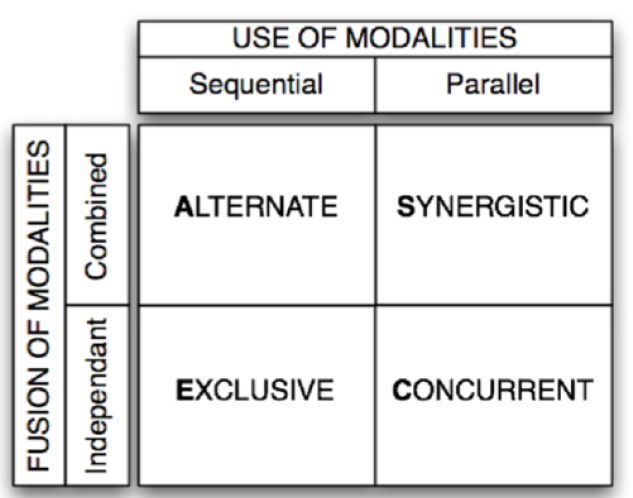
\includegraphics[scale=0.9]{casecare}
\caption{The CASE model}
\label{case-model}
\end{figure}
\newline
The \textit{CASE} model classified the machine-side of the fusion, now the \textit{CARE} model is about the human-side of fusion and classifies the usability properties: in our application, the two modalities are complementary. We need to use both of them at the same time to use correctly the application. 

\subsection{Fusion and fission}
We use \textit{decision-level fusion}: we merge lately the two modalities (the gaze position and the key pressing) because they are weakly coupled. On the fission side, it is a bit hard to have two different outputs for the user: we kept the feedback visual by highlighting the gazed-at element and by letting the menus appear directly upon a key press.  

\section{Architecture}

\subsection{Hardware} \label{hardware}
The main hardware used for this project is a \textit{Tobii EyeTracker 4C}, a USB eye tracker using an infrared camera to track the gaze position and translate it to the screen. This system is relatively low cost and works well enough for many usages, as unlike more expensive systems, the point of the \textit{4C} isn't to properly track every single movement but more to determine the different areas gazed upon. 
And for our project we will use it in coordination with a standard keyboard.

\subsection{Software}
To be able to access the \textit{Tobii} gaze data, we used the \textit{Tobii Core Standard Development Kit} \footnote{\url{https://developer.tobii.com/tobii-core-sdk/}} 
and its provided \textit{API}s. 
We then decided not to implement a plugin for an already existing text editor but rather to create our own one. The \textit{Windows Presentation Foundation}\footnote{\url{https://msdn.microsoft.com/fr-fr/library/aa970268(v=vs.100).aspx}} was all we needed: windows creation with built-in text fields and style modification. The \textit{WPF} uses the \textit{XAML} language. \footnote{Our code and a released version is available on \href{https://github.com/marom17/E.A.T./releases/tag/1.0.5}{GitHub} under the MIT license}

\subsection{Implementation}
The integration of the \textit{Tobii} in our application is quiet easy. There is a good synergy between \textit{WPF} and the \textit{Tobii SDK}. We can add some parameter to the element of a window to add the capacity to use the eye tracker.

\begin{lstlisting}[frame=single, language=XML]
<Button x:Name="validation"
wpf:Behaviors.IsActivatable="True"
wpf:Behaviors.IsTentativeFocusEnabled="True"
wpf:Behaviors.Activated="activation_function">
\end{lstlisting}

The above example of code allows a button to be activated by the eye tracker. When it is activated, it calls the function \textit{activation\_function}.

\subsubsection{In the app}
We use the eye tracker in our application as follows:
\begin{itemize}
\item Scroll the text
\item Quick menu for the main function of the application
\item Select the style of the text
\item Correct spelling mistakes
\end{itemize}

\section{Data analysis}

\subsection{Hypothesis}
We hope to see a significant amelioration in the text editing quality by using our application. Therefore we can formulate our null hypothesis as follows: 
\[H_0: \text{There is no increase in speed by editing text with the eye tracker.}\] 
along with the alternative hypothesis: 
\[H_1: \text{Editing text with eye tracker support is faster than without it.}\]

\subsection{Protocol}

\subsubsection{Discovery}
After giving the user a brief introduction on eye tracking with the \textit{4C} we go through the calibration process and let them play a bit with the system. Then we introduce our software and let them play a bit with it to get used to it.

\subsubsection{Test}
The user was first asked to copy a given short text with a precise formatting, e.g. different fonts and font sizes (see Appendix \ref{Test}). This was done either with the eye-tracking interface or with the classical one. \\
We then swapped to the other modality choice and asked the user to repeat the task on the same text. \\
The time for both parts was measured. 

Originally we planed also to check the usability to use eye tracking on text editing, but after the first trials our method didn't work.


\subsubsection{Evaluation}
The user then filled a form to gather their feedback and impression. This form touched upon personal preferences, potential (does the user feel like he could become more proficient with more experience), issues and ideas. 

\subsection{Experiment and results}

\subsubsection{Quantitative measures}
Nobody was faster using the eye tracking. And for some users the eye tracking was nearly 3 time slower (see Table \ref{timetable}.) With a mean of respectively 232.875 and 404.375, the mouse still reigns over the eye tracking in our sample. T-Test only reinforce this, clearly showing the favour towards mouse tracking. 

\begin{lstlisting}[frame=single, language=R]
Welch Two Sample t-test
t = -3.4619, df = 13.545, p-value = 0.003984

mean of x mean of y 
  232.875   404.375 

#With x for Mouse usage and y for Eye tracker.
\end{lstlisting}

\begin{table}
\centering
\begin{tabular}{c|c|c}
Mouse & Eye tracking&Ratio E/M\\
\hline
206&434&2.11\\
184&254&1.48\\
270&520&1.93\\
147&411&2.79\\
169&301&1.78\\
398&562&1.41\\
165&316&1.92\\
324&437&1.35\\
\end{tabular}
\caption{Results in second}
\label{timetable}
\end{table}


\subsubsection{User feedback} \label{feedback}
In the user feedback given in the form, the trend of "\textit{Keyboard and mouse are a better combination of modalities for text editing}" is a bit toned down: all users rated all three impressions -- ease of use, swiftness, comfort -- with at least an \textit{Average} rating, and most votes were between \textit{Average} and \textit{Excellent}. The preference of users still go to the keyboard and mouse combination in most cases. \\
Even though all but one of them felt that they experienced issues with eye tracking, what really gives us hope for such a project is that no user thinks he cannot improve, even if some may not be sure about it. 
See Appendix \ref{FormResults}

\section{Conclusion}

\subsection{Review}

In this whole experiment, we have seen that our interface is not yet better than the conventional interface. We believe, as do most of the users, that our usage of eye tracking can get better and that interfaces using eye tracking in some way will one day make text editing easier for everybody. \\
One fact that we observed is that the users often had their first contact with Eye tracking only a few minutes before our experiment. This may explain some of the difference for the time needed to edit text with eye tracking. As said in section \ref{feedback} about feedback, the users mostly thought they could improve. It could be interesting to make this experiment again with more experimented subjects. \\
Our experience was a bit exaggerated, as we forced the user to do multiple style changes in a row; which is not usual in the documents one can easily type. This factor causes the time difference to be higher than it would have with less editing and more typing, which is not affected by eye tracking. 
It is still to be noted that all users did not use the mouse at all for editing with eye tracking. This is a positive note for our interface. 
One must keep in mind the fact that our application was meant to be a quick testing tool, not a complete standalone text editor. Therefore it suffered from some problems that would have been avoided by creating a plug in for an existing editor. \\
We can still extract a few reasons that made our application not fully benefit from eye tracking -- and some possible solutions to them: \\
Our text editor was quite basic: we adapted a bit the size of some menus, but a list menu does not feel really adequate for eye selection. We could adapt the menus, for example with circular menus or bigger tiles. As already explained in section \ref{hardware}, the \textit{Tobii Eye Tracker 4C} is not exceptionally precise. Excluding calibration problems, we still need to adapt our application to the device's capabilities.\\
To follow on the last point, we kept some simple shortcuts for menu generation and simple element disposition. It could be possible to either find better dispositions and shortcuts by testing different configurations or by allowing the user to choose them to fit his preferences. One example is the spell checker feedback: by opening the spell check, the user masks the text and does not see the sentence being corrected. We could display the few words before and after the wrongly spelled word in the suggestion box. 

\subsection{Personal feedback}
After some discussion, it appeared that all three of us had some great pleasure in doing this project! We discovered the \textit{Tobii Eye Tracker}, we had fun playing with it, and seeing our application work with eye control was a great reward. The \textit{WPF} also turned to be really practical and easy to use, it's a tool we may use again in the future. \\
\newpage
\appendix
\section{Feedback form results}
\label{FormResults}
\begin{figure}[H]
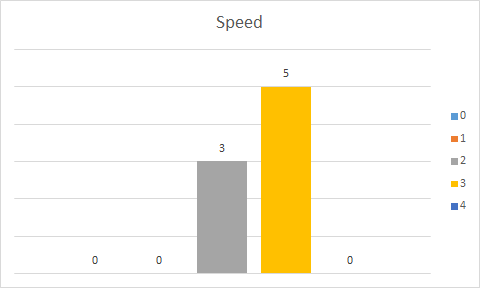
\includegraphics[scale =.59]{Speed}
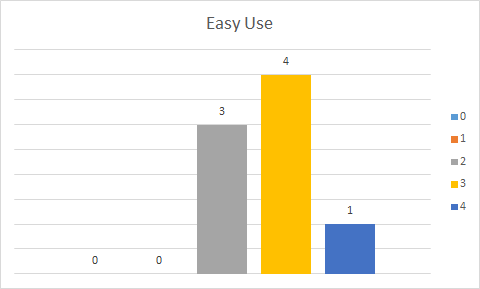
\includegraphics[scale =.59]{EaseOfUse}
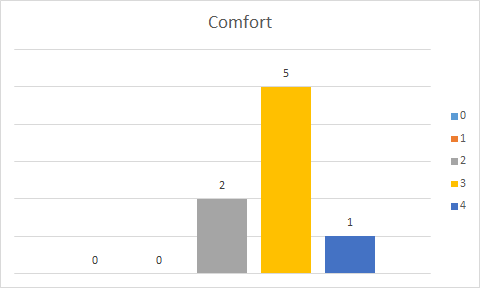
\includegraphics[scale =.59]{Comfort}
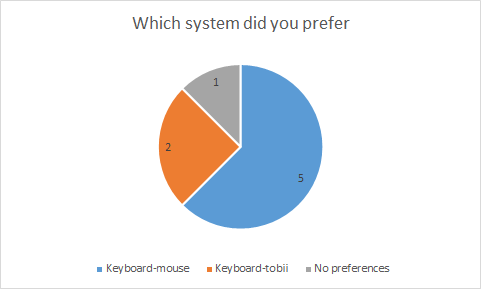
\includegraphics[scale =.59]{Preference}
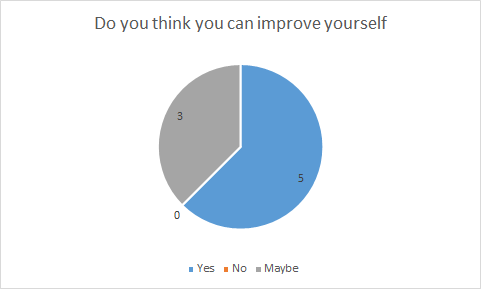
\includegraphics[scale =.59]{Improvement}
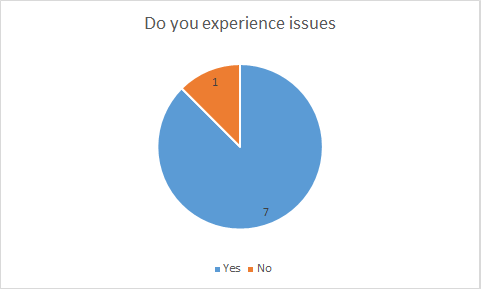
\includegraphics[scale =.59]{Issues}
\end{figure}
\newpage
\section{Text for the test}
\label{Test}
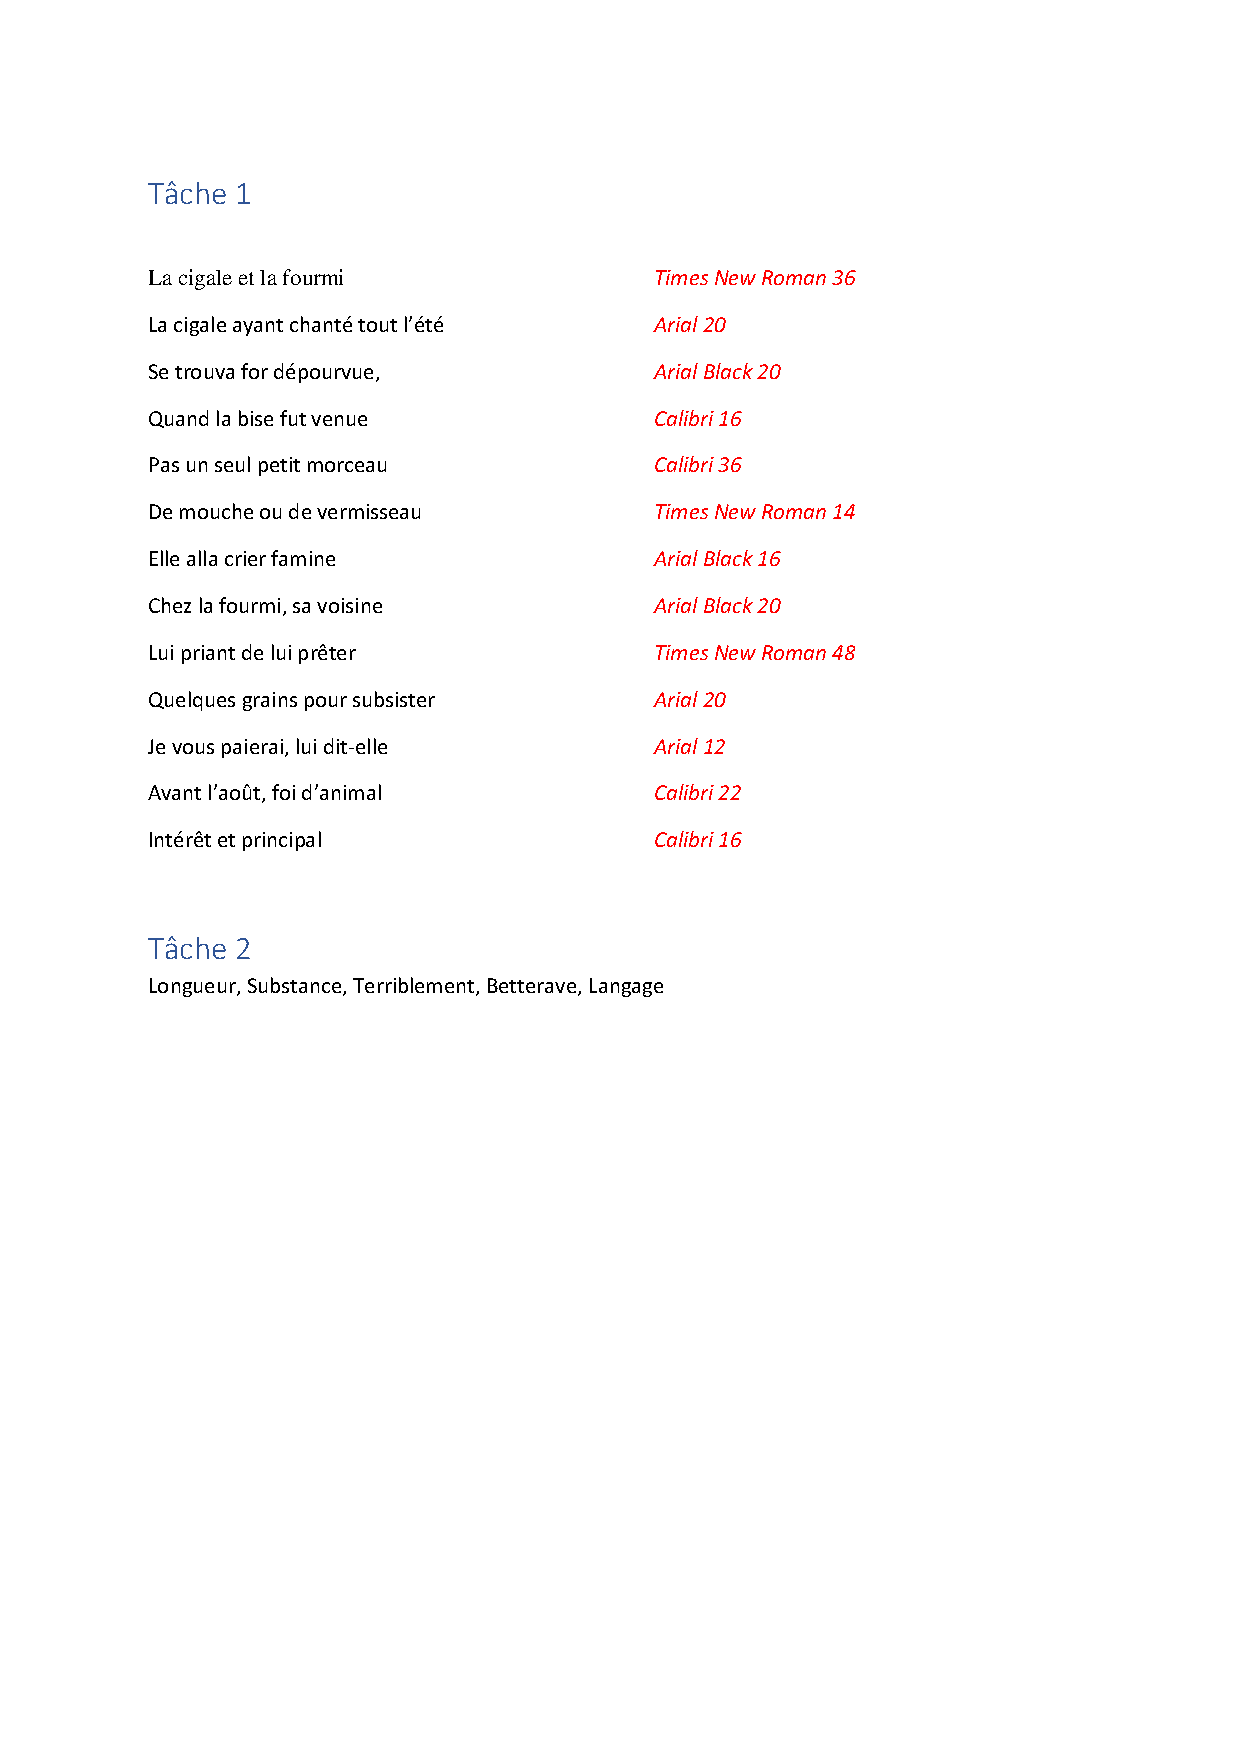
\includepdf{new_protocol_FR.pdf}
 
\end{document}

 